\documentclass[12pt,a4paper]{article}
\usepackage{geometry}
\usepackage{tikz}
\usetikzlibrary{positioning}
\geometry{margin=2.5cm}
\usepackage{enumitem}
\usepackage{amsmath}
\usepackage{float}
\usepackage{fancyhdr}
\usepackage{titlesec}

\geometry{margin=2.5cm}
\pagestyle{fancy}
\fancyhf{}
\rhead{Ujian Struktur Data}
\lhead{Nama Mahasiswa}
\rfoot{Halaman \thepage}
\titleformat{\section}{\large\bfseries\uppercase}{}{0em}{}
\titlespacing*{\section}{0pt}{2ex plus 0.5ex minus 0.2ex}{1ex plus 0.3ex}

\begin{document}

\begin{center}
    {\Large \textbf{Jawaban UAS Struktur Data}} \\
    \vspace{0.5cm}
    Matakuliah: Struktur Data \\
    Dosen: Uro Abdulrohim, MT. \\
    \vspace{0.5cm}
    Nama: Rifqi Fadil Fahrial\\
    NIM: 1222646
\end{center}

\vspace{1cm}

\section{Soal 1: Cara Kerja Queue Menggunakan Array}

Queue adalah struktur data yang bekerja berdasarkan prinsip FIFO (First In First Out), artinya elemen yang pertama dimasukkan akan keluar lebih dulu.

Untuk implementasi queue menggunakan array, dibutuhkan dua variabel penunjuk:

    
- \texttt{front}: menunjuk ke elemen paling depan.
    
- \texttt{rear}: menunjuk ke elemen paling belakang.


Operasi utama:
    
- \texttt{enqueue(x)}: menambahkan elemen di posisi \texttt{rear}.
    
- \texttt{dequeue()}: menghapus elemen dari posisi \texttt{front}.

\subsection{Ilustrasinya}

Pada awalnya, queue kosong, sehingga `front = 0` dan `rear = -1`.

\begin{center}
    \begin{tikzpicture}[node distance=1cm]
        % Define styles
        \tikzstyle{array} = [draw, minimum width=1.5cm, minimum height=1cm];
        \tikzstyle{label} = [above, font=\small];

        % Draw array cells
        \node[array] (cell0) {};
        \node[array, right=of cell0] (cell1) {};
        \node[array, right=of cell1] (cell2) {};
        \node[array, right=of cell2] (cell3) {};
        \node[array, right=of cell3] (cell4) {};

        % Add labels for indices
        \node[label] at (cell0.north) {0};
        \node[label] at (cell1.north) {1};
        \node[label] at (cell2.north) {2};
        \node[label] at (cell3.north) {3};
        \node[label] at (cell4.north) {4};

        % Add front and rear pointers
        \node[below=of cell0, font=\small] (front) {front = 0};
        \node[below=of cell4, font=\small] (rear) {rear = -1};

        % Arrows for front and rear
        \draw[->, thick] (front) -- (cell0.south);
        \draw[->, thick] (rear) -- ++(0,-0.5) node[below] {\textbf{(kosong)}};
    \end{tikzpicture}
  \end{center}
\subsection{Setelah Enqueue Pertama (Masukkan 'A')}

Setelah memasukkan elemen pertama ('A'), `rear` menjadi 0.

\begin{center}
    \begin{tikzpicture}[node distance=1cm]
        % Define styles
        \tikzstyle{array} = [draw, minimum width=1.5cm, minimum height=1cm];
        \tikzstyle{label} = [above, font=\small];

        % Draw array cells
        \node[array] (cell0) {A};
        \node[array, right=of cell0] (cell1) {};
        \node[array, right=of cell1] (cell2) {};
        \node[array, right=of cell2] (cell3) {};
        \node[array, right=of cell3] (cell4) {};

        % Add labels for indices
        \node[label] at (cell0.north) {0};
        \node[label] at (cell1.north) {1};
        \node[label] at (cell2.north) {2};
        \node[label] at (cell3.north) {3};
        \node[label] at (cell4.north) {4};

        % Add front and rear pointers
        \node[below=of cell0, font=\small] (front) {front = 0};
        \node[below=of cell0, font=\small, xshift=2cm] (rear) {rear = 0};

        % Arrows for front and rear
        \draw[->, thick] (front) -- (cell0.south);
        \draw[->, thick] (rear) -- (cell0.south);
    \end{tikzpicture}
\end{center}

\subsection{Setelah Enqueue Kedua (Masukkan 'B')}

Setelah memasukkan elemen kedua ('B'), `rear` menjadi 1.

\begin{center}
    \begin{tikzpicture}[node distance=1cm]
        % Define styles
        \tikzstyle{array} = [draw, minimum width=1.5cm, minimum height=1cm];
        \tikzstyle{label} = [above, font=\small];

        % Draw array cells
        \node[array] (cell0) {A};
        \node[array, right=of cell0] (cell1) {B};
        \node[array, right=of cell1] (cell2) {};
        \node[array, right=of cell2] (cell3) {};
        \node[array, right=of cell3] (cell4) {};

        % Add labels for indices
        \node[label] at (cell0.north) {0};
        \node[label] at (cell1.north) {1};
        \node[label] at (cell2.north) {2};
        \node[label] at (cell3.north) {3};
        \node[label] at (cell4.north) {4};

        % Add front and rear pointers
        \node[below=of cell0, font=\small] (front) {front = 0};
        \node[below=of cell1, font=\small, xshift=2cm] (rear) {rear = 1};

        % Arrows for front and rear
        \draw[->, thick] (front) -- (cell0.south);
        \draw[->, thick] (rear) -- (cell1.south);
    \end{tikzpicture}
\end{center}

\subsection{Setelah Dequeue Pertama (Hapus 'A')}

Setelah menghapus elemen pertama ('A'), `front` menjadi 1.

\begin{center}
    \begin{tikzpicture}[node distance=1cm]
        % Define styles
        \tikzstyle{array} = [draw, minimum width=1.5cm, minimum height=1cm];
        \tikzstyle{label} = [above, font=\small];

        % Draw array cells
        \node[array] (cell0) {};
        \node[array, right=of cell0] (cell1) {B};
        \node[array, right=of cell1] (cell2) {};
        \node[array, right=of cell2] (cell3) {};
        \node[array, right=of cell3] (cell4) {};

        % Add labels for indices
        \node[label] at (cell0.north) {0};
        \node[label] at (cell1.north) {1};
        \node[label] at (cell2.north) {2};
        \node[label] at (cell3.north) {3};
        \node[label] at (cell4.north) {4};

        % Add front and rear pointers
        \node[below=of cell1, font=\small] (front) {front = 1};
        \node[below=of cell1, font=\small, xshift=2cm] (rear) {rear = 1};

        % Arrows for front and rear
        \draw[->, thick] (front) -- (cell1.south);
        \draw[->, thick] (rear) -- (cell1.south);
    \end{tikzpicture}
\end{center}

\subsection{Setelah Enqueue Ketiga (Masukkan 'C')}

Setelah memasukkan elemen ketiga ('C'), `rear` menjadi 2.

\begin{center}
    \begin{tikzpicture}[node distance=1cm]
        % Define styles
        \tikzstyle{array} = [draw, minimum width=1.5cm, minimum height=1cm];
        \tikzstyle{label} = [above, font=\small];

        % Draw array cells
        \node[array] (cell0) {};
        \node[array, right=of cell0] (cell1) {B};
        \node[array, right=of cell1] (cell2) {C};
        \node[array, right=of cell2] (cell3) {};
        \node[array, right=of cell3] (cell4) {};

        % Add labels for indices
        \node[label] at (cell0.north) {0};
        \node[label] at (cell1.north) {1};
        \node[label] at (cell2.north) {2};
        \node[label] at (cell3.north) {3};
        \node[label] at (cell4.north) {4};

        % Add front and rear pointers
        \node[below=of cell1, font=\small] (front) {front = 1};
        \node[below=of cell2, font=\small, xshift=2cm] (rear) {rear = 2};

        % Arrows for front and rear
        \draw[->, thick] (front) -- (cell1.south);
        \draw[->, thick] (rear) -- (cell2.south);
    \end{tikzpicture}
  \end{center}


\vspace{1cm}

\section{Soal 2: Definisi Struktur Data Double Linked List}
\begin{figure}[H]
  \begin{center}
    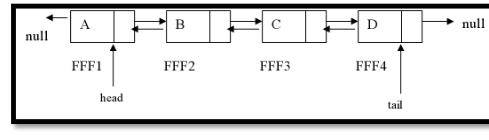
\includegraphics[width=0.8\textwidth]{images/gambar2.jpg}
  \end{center}
\end{figure}
Struktur data yang ditampilkan di gambar menunjukan sebuah sistem double linked list yang menunjukan sistem pointer yang menghubungkan antar node secara bolak balik sehingga mempercepat pencarian data secara traversal (bolak balik), untuk variabel yang diperlukan adalah 
\begin{itemize}
  \item Data yang disimpan 
  \item Pointer menunjuk ke depan (next) 
  \item pointer menunjuk ke belakang (prev)
\end{itemize}
Struktur node untuk double linked list:

\begin{verbatim}
struct Node {
    int data;
    Node* prev;
    Node* next;
};
\end{verbatim}



\vspace{1cm}

\section{Soal 3: Prosedur Inisialisasi Double Linked List}

untuk menginisialisasi double linked list, maka perlu menambahkan variabel baru yang dapat menunjukkan data yang paling depan (head) dan data paling belakang (tail). maka dapat di inisialisasikan sebagai berikut:

\begin{verbatim}
void initList(Node*& head, Node*& tail) {
    head = NULL;
    tail = NULL;
}
\end{verbatim}

\vspace{1cm}

\section{Soal 4: Algoritma Penambahan Data di Depan Double Linked List}

Algoritma penambahan di depan:

\begin{verbatim}
void insertDepan(Node*& head, Node*& tail, int nilai) {
    Node* baru = new Node;
    baru->data = nilai;
    baru->prev = NULL;
    baru->next = NULL;

    if (head == NULL) { // Jika list kosong
        head = baru;
        tail = baru;
    } else { // Jika tidak kosong
        baru->next = head;
        head->prev = baru;
        head = baru;
    }
}
\end{verbatim}

\vspace{1cm}

\section{Soal 5: Traversal Pada Tree (Pre-order, In-order, Post-order)}

Diberikan struktur pohon sebagai berikut:

\begin{figure}[H]
  \begin{center}
    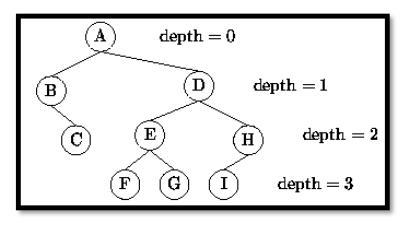
\includegraphics[width=0.8\textwidth]{images/gambar1.jpg}
  \end{center}
\end{figure}



Hasil traversal:
\subsection*{1. Pre-order Traversal (Root-Left-Right)}
\begin{itemize}
    \item \textbf{Aturan:} Kunjungi node akar (Root), lalu kunjungi sub-pohon kiri (Left) secara rekursif, kemudian kunjungi sub-pohon kanan (Right) secara rekursif.
    \item \textbf{Hasilnya} A $\rightarrow$ B $\rightarrow$ C $\rightarrow$ D $\rightarrow$ E $\rightarrow$ F $\rightarrow$ G $\rightarrow$ H $\rightarrow$ I
\end{itemize}

\subsection*{2. In-order Traversal (Left-Root-Right)}
\begin{itemize}
    \item \textbf{Aturan:} Kunjungi sub-pohon kiri (Left) secara rekursif, lalu kunjungi node akar (Root), kemudian kunjungi sub-pohon kanan (Right) secara rekursif.
    \item \textbf{Hasilnya} C $\rightarrow$ B $\rightarrow$ F $\rightarrow$ E $\rightarrow$ G $\rightarrow$ A $\rightarrow$ D $\rightarrow$ H $\rightarrow$ I
\end{itemize}

\subsection*{3. Post-order Traversal (Left-Right-Root)}
\begin{itemize}
    \item \textbf{Aturan:} Kunjungi sub-pohon kiri (Left) secara rekursif, lalu kunjungi sub-pohon kanan (Right) secara rekursif, kemudian kunjungi node akar (Root).
    \item \textbf{Hasilnya} C $\rightarrow$ F $\rightarrow$ G $\rightarrow$ E $\rightarrow$ I $\rightarrow$ H $\rightarrow$ D $\rightarrow$ B $\rightarrow$ A
\end{itemize}

    


\vspace{1cm}

\section{Soal 6: Deklarasi Struktur Data untuk Tree}

Struktur node untuk tree:

\begin{verbatim}
struct Node {
    int data;
    Node* kiri;
    Node* kanan;
};

Node* root = NULL;
\end{verbatim}


Variabel yang dibutuhkan adalah : \\ 
\begin{enumerate}
  \item Variabel data yang disimpan, dalam kasus ini adalah integer 
  \item Pointer yang menunjuk ke node sama yang dalam kasus tree ini mengarah ke arah kiri dan kanan karena ada dua arah yang dapat diakses untuk, dengan value NULL sebagai default yang berarti value kosong / tidak ada / tidak dibuat
  \item Variabel root yang mana menginisialisasi kan Tree data structure yang menjadi awal dari pencarian data.
\end{enumerate}
\vspace{1cm}

\section{Soal 7: Implementasi Class TKalkulator dalam Bahasa C++}

Implementasi class \texttt{TKalkulator}:

\begin{verbatim}
#include <iostream>
using namespace std;

class TKalkulator {
private:
    int opr1;
    int opr2;
    int hasil;

public:
    void setBilangan1(int op) { opr1 = op; }
    void setBilangan2(int op) { opr2 = op; }

    int getBilangan1() { return opr1; }
    int getBilangan2() { return opr2; }
    int getHasil() { return hasil; }

    int Penjumlahan() {
        hasil = opr1 + opr2;
        return hasil;
    }

    int Pengurangan() {
        hasil = opr1 - opr2;
        return hasil;
    }

    int Perkalian() {
        hasil = opr1 * opr2;
        return hasil;
    }

    int PembagianBulat() {
        if (opr2 != 0)
            hasil = opr1 / opr2;
        else {
            cout << "Error: Pembagi nol!" << endl;
            hasil = 0;
        }
        return hasil;
    }

    int PembagianSisa() {
        if (opr2 != 0)
            hasil = opr1 % opr2;
        else {
            cout << "Error: Pembagi nol!" << endl;
            hasil = 0;
        }
        return hasil;
    }
};

int main() {
    TKalkulator calc;
    calc.setBilangan1(10);
    calc.setBilangan2(3);

    cout << "Penjumlahan: " << calc.Penjumlahan() << endl;
    cout << "Pengurangan: " << calc.Pengurangan() << endl;
    cout << "Perkalian: " << calc.Perkalian() << endl;
    cout << "Pembagian Bulat: " << calc.PembagianBulat() << endl;
    cout << "Pembagian Sisa: " << calc.PembagianSisa() << endl;

    return 0;
}
\end{verbatim}

\end{document}
